\chapter{\textbf{Reconnaissance Optique de Caractères}}
    \section{Introduction}
    Si les humains peuvent très facilement reconnaître les caractères sur un document, notamment une image est chose facile, ce n’est pas le cas pour les ordinateurs. En effet, comme nous l’avons vu au chapitre précédent, une image pour un ordinateur n’est qu’une série de points. Le besoin croissant de numérisation des documents imprimés a fait naître une nouvelle technologie qu’on appelle généralement l'OCR. Ce chapitre nous permettra de comprendre ce qu'est réellement cette technologie d’abord, ensuite nous présenterons les phases d’un processus d’OCR et nous terminerons par les outils utilisés pour réaliser l’OCR.
    
    \section{Définition}
L'OCR ou encore la reconnaissance optique de caractères est une technologie complexe qui convertit les images contenant du texte en formats avec du texte modifiable. Il permet de traiter des livres numérisés, des captures d'écran et des photos contenant du texte et d'obtenir des documents modifiables tels que des fichiers TXT, DOC ou PDF.
\begin{figure}[H]
    \centering
    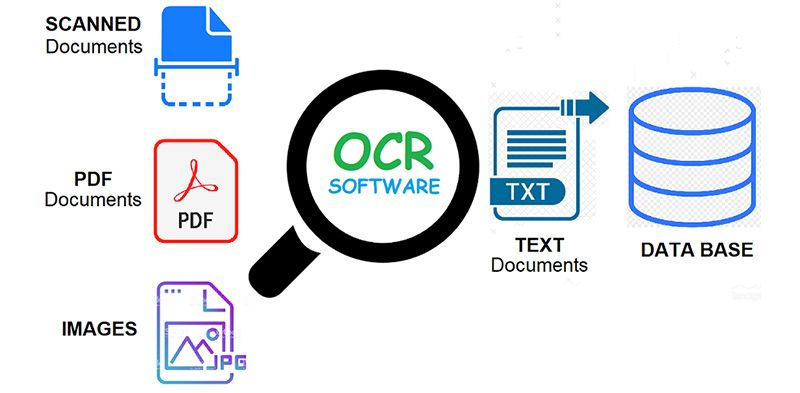
\includegraphics[scale=0.25]{OCR}
    \caption{Processus d'OCR}
\end{figure}
    \section{Phases d'OCR}
Pour arriver à extraire le texte se trouvant sur un document, la technologie OCR le fait passer par une succession de plusieurs étapes.
    \subsection{Prétraitement}
    L’objectif de cette étape est d’améliorer la qualité de l’image et de faciliter son traitement pour de meilleurs résultats. Pour cela, on utilise quelques méthodes comme:
    \begin{itemize}
        \item[•]\textbf{La binarisation}: Il s'agit de convertir une image en couleur qui est en trois dimensions en une image bidimensionnelle noir sur blanc. Pour cela, on passe par une étape intermédiaire
        appelée le \textit{grayscaling} qui convertit l'image en gris et en utilisant le seuillage sur l'image obtenue pour aboutir à une image en noir et blanc.
        \item[•]\textbf{Le redressement}: Lors du processus de numérisation des documents, il peut y arriver
        quelques déformations sur le document numérisé obtenu. Ces déformations peuvent être des
        inclinaisons du texte. Cette étape permet de redresser l'image afin que les textes par exemple
        soient placées horizontalement.
        \item[•]\textbf{Le zonage}: Il permet de selectionner la partie de l'image où l'on veut extraire les informations.
        \item[•]\textbf{Le suppression des bruits}: Ici on enlève les éléments qui peuvent être considérés comme du bruit de l'image. Ceci peut des lignes verticaux, horizontaux, obliques, des points en arrière plan.
        \item[•]\textbf{L'amincissement et la squelettisation }: Il permet d'uniformiser la taille du texte dans l'image.   
    \end{itemize}

    \subsection{Segmentation}
    Le but de cette phase est d'isoler les lignes et les  caractères se trouvant sur l'image. Il existe donc trois types de segmentation:
        \begin{itemize}
            \item[•]\textbf{La segmentation des lignes}:L'objectif principal de ce type est de déterminer les coordonnées des lignes dans l'image, ce qui peut diviser l'image en lignes. L’idée est que, si nous projetons horizontalement l'image binaire, les lignes qui ont les pixels de texte ont des pics plus élevés, en raison du plus grand nombre de pixels de premier plan et les lignes qui ont l'espacement entre les lignes ont des pics plus faibles, en raison du plus grand nombre de pixels d'arrière-plan. 
            \item[•]\textbf{La segmentation des mots}:L'objectif principal de ce type est de déterminer où nous devons segmenter l'image pour séparer les mots. L’idée est la même que l'étape précédente, mais le seul changement est ici que nous projetons l'image verticalement parce que nous séparons les mots verticalement. Les colonnes qui ont les pixels de texte ont des pics plus élevés, en raison de plus de nombre de pixels de premier plan et les colonnes qui ont l'espace entre les mots contiennent des pics plus faibles, en raison de plus de nombre de pixels d'arrière-plan.
            \item[•]\textbf{La segmentation des caractères}:la tâche de la segmentation au niveau des caractères consiste à séparer les caractères uniques (comme les alphabets, les chiffres et autres symboles) des mots qui sont séparés de l'étape précédente.
        \end{itemize}
    Pour la segmentation des images, la technique la plus utilisée est la projection histogramme, on cite deux types de projection :
        \begin{itemize}
            \item[•]\textbf{La projection horizontale} : Utilisée dans la segmentation au niveau des lignes.
            \item[•]\textbf{La projection verticale}: Utilisée dans la segmentation au niveau des mots et des caractères.
        \end{itemize}
    \subsection{Reconnaissance de caractères}
    Le but est d'identifier numériquement le caractères qui est en image. Pour y parvenir, il existe des techniques de reconnaissance qui peuvent classées en trois grands groupes:
        \begin{enumerate}
            \item \textbf{La classification par caractéristiques (Features)}: une forme à reconnaître est représentée par un vecteur de valeurs numériques - appelées features en anglais - calculées à partir de cette forme. Le nombre de features est de l'ordre de 100 à 300. Si les features sont bien choisies, une classe de caractères (par exemple l'ensemble des A majuscules) sera représentée par un « nuage » contigu de points dans l'espace vectoriel des features. Le rôle du classificateur est de déterminer à quel nuage (donc à quelle classe de caractères) la forme à reconnaitre appartient le plus vraisemblablement. La classification fait généralement appel à divers types de réseaux de neurones artificiels entrainés sur de vastes bases de formes possibles.
            \item \textbf{Les méthodes métriques} : consistent à comparer directement la forme à reconnaître, au moyen d'algorithmes de distance, avec un ensemble de modèles appris. Ce type de méthode est peu utilisé et peu valorisé par les chercheurs, car souvent plus naïf et vraisemblablement moins efficace que les méthodes à base de features.
            \item \textbf{Les méthodes statistiques}: dans le domaine de la reconnaissance d'écriture manuscrite, il est fréquemment fait appel aux méthodes probabilistes comme les chaînes de Markov.\cite{wikiOCR}
        \end{enumerate}

    \subsection{Post-traitement}
    L'objectif de cette phase est de reduire les erreurs de reconnaissance. On utilise à cet effet des méthodes linguistiques et contextuelles pour identifier les mauvaises reconnaissances et proposer une éventuelle correction. 
    \section{Outils}
De nombreuses \acrshort{api} et bibliothèques ont été développées pour effectuer les opérations d’OCR sur les documents. Parmi elles, nous pouvons citer:

\begin{itemize}
    \item \textbf{Tesseract}:c’est un moteur de reconnaissance optique de caractères écrit en C et C++ pour divers systèmes d'exploitation (Linux, Windows et Mac OS X). Il s'agit d'un logiciel gratuit, publié sous la licence Apache, et le développement est parrainé par Google depuis 2006. En 2006, Tesseract était considéré comme l'un des moteurs OCR open source les plus précis. Avec la version 4, un moteur et des modèles OCR basés sur LSTM (Long-Short Term Memory) pour de nombreuses langues et scripts supplémentaires ont été ajoutés, portant ainsi le nombre de langues traitées à 116.
    \item \textbf{EasyOCR}: comme Tesseract, EasyOCR est une bibliothèque  open source d’OCR. Développé par JaidedAI , il prend en charge plus de 80 langues et tous les scripts d'écriture courants, notamment le latin, le chinois, l'arabe, le cyrillique, etc. Par rapport à Tesseract, il possède l’avantage d’être rapide lors d’une exécution avec le GPU.
    \item \textbf{MLKit Text Recognition}: 
    C’est API développé par Google pour l’OCR. Elle est principalement utilisée dans les applications mobiles et prend uniquement en compte les caractères latins.
    
\end{itemize}


    \section{Conclusion}
    L’OCR est une technologie qui permet aux ordinateurs de lire les documents comme les humains. Elle s’étend sur 4 principales phases dont l’une des plus cruciales est la reconnaissance des caractères. Des méthodes ont été proposées pour réussir de plus en plus cette phase. L’une des méthodes qui a fait ces preuves est l’apprentissage automatique ou le Machine Learning. Ce concept qui s’est répandu dans le monde de l’informatique sera l’objet du prochain chapitre.